%% \documentclass[handout,t]{beamer} % HANDOUT
\documentclass[handout,notes=show,t]{beamer} % NOTES
%% \documentclass[t]{beamer} % SLIDES

\usetheme{ZipfR}
\usepackage{beamer-tools}

\input{lib/math}  % basic mathematical notation
\input{lib/stat}  % notation for probability theory and statistics
\input{lib/vector}% convenience macros for vectors and matrices

%%%
%%% local configuration adjustments
%%%

%%% You can change pre-defined colours here, override built-in macros from the
%%% style definition and standard library, as well as define macros needed by
%%% all local documents.

%%% e.g. adjust counterpoint (dark green) for data projectors where greens are
%%% far too bright, as well as green component of light colour and pure green
%%% (of course, it's a better solution to adjust the gamma settings of your monitor)
%%
%% \definecolor{counterpoint}{rgb}{.1, .3, 0}
%% \definecolor{light}{rgb}{.45, .3, .55}
%% \definecolor{puregreen}{rgb}{0, .35, 0}

%% ----- extra packages we need to load

\usepackage{tikz}
\usepackage{alltt}              % code examples with nicely formatted comments


%% ----- automatically show TOC reminder at beginning of each subsection
\AtBeginSubsection[]
{
  \begin{frame}
    \frametitle{Outline}
    \tableofcontents[current,currentsubsection]
  \end{frame}
}

%% ----- some useful macros for R examples

%% > plot(x,y)      \REM{this produces a scatterplot}
\newcommand{\REM}[2][\small]{\textsf{#1\color{primary}\# #2}}

%% nice colour for R output: \begin{Rout} .. \end{Rout}
%% -- ugly hack: I'm sure theres a better way to do this
\newenvironment{Rout}[1][\footnotesize]{%
  \begin{footnotesize}#1\color{dsmblue}\bfseries}{%
  \color{black}\mdseries\end{footnotesize}}

%% ----- other macros -----

%% \IV{condition} ... indicator variable
\newcommand{\IV}[1]{I_{[#1]}}

%% \dpi ... integration over pi
\newcommand{\dpi}[0]{\dX{\pi}} % local adjustments to configuration and macros

%%%%%%%%%%%%%%%%%%%%%%%%%%%%%%%%%%%%%%%%%%%%%%%%%%%%%%%%%%%%%%%%%%%%%%
%% Titlepage

\title[Productivity in small samples]{The impossibility of measuring productivity\\ in small samples}
\subtitle{}
\author[Stefan Evert]{Stefan Evert\\ FAU Erlangen-Nürnberg}
\date[MISC | 18 May 2018]{\small MISC Workshop @ HU Berlin\\18 May 2018}

\begin{document}

\pgfdeclareimage[width=30mm]{kallimachos-logo}{img/logo_kallimachos}
\logo{\pgfuseimage{kallimachos-logo}}

\frame{\titlepage}
\hideLogo{}
\AtBeginSubsection[]{}

%%%%%%%%%%%%%%%%%%%%%%%%%%%%%%%%%%%%%%%%%%%%%%%%%%%%%%%%%%%%%%%%%%%%%%%%
\section{Notation}
\subsection{and basic concepts}

\newcommand{\TC}[1]{\counterpoint{\emph{#1}}}
\newcommand{\TL}[1]{\light{\emph{#1}}}
\newcommand<>{\TA}[1]{\light{\counterpoint#2{\emph{#1}}}}

\begin{frame}
  \frametitle{Tokens \& types}

  our sample: \TC{recently}, \TC{very}, \TC{not}, \TC{otherwise}, \TC{much}, \TC{very},
  \TC{very}, \TC{merely}, \TC{not}, \TC{now}, \TC{very}, \TC{much},
  \TC{merely}, \TC{not}, \TC{very}

  \begin{itemize}
  \item $N = 15$: number of \hh{tokens} = sample size
  \item $V = 7$: number of distinct \hh{types} = \h{vocabulary size}\\
    (\TC{recently}, \TC{very}, \TC{not}, \TC{otherwise}, \TC{much}, \TC{merely}, \TC{now})
  \end{itemize}

  \onslide<2->
  \begin{columns}[c]
    \begin{column}{5cm}
      \centering
      \h{type-frequency list}

      \begin{tabular}{l|c}
        $w$ & $f_w$ \\
        \hline
        \TC{recently} & 1 \\ 
        \TC{very}     & 5 \\
        \TC{not}      & 3 \\ 
        \TC{otherwise}& 1 \\ 
        \TC{much}     & 2 \\ 
        \TC{merely}   & 2 \\ 
        \TC{now}      & 1 
      \end{tabular}
    \end{column}
    \begin{column}{5cm}
      
    \end{column}
  \end{columns}
\end{frame}

\begin{frame}
  \frametitle{Zipf ranking}

  our sample: \TC{recently}, \TC{very}, \TC{not}, \TC{otherwise}, \TC{much}, \TC{very},
  \TC{very}, \TC{merely}, \TC{not}, \TC{now}, \TC{very}, \TC{much},
  \TC{merely}, \TC{not}, \TC{very}

  \begin{itemize}
  \item $N = 15$: number of \hh{tokens} = sample size
  \item $V = 7$: number of distinct \hh{types} = \h{vocabulary size}\\
    (\TC{recently}, \TC{very}, \TC{not}, \TC{otherwise}, \TC{much}, \TC{merely}, \TC{now})
  \end{itemize}

  \begin{columns}[c]
    \begin{column}{5cm}
      \centering
      \h{Zipf ranking}

      \begin{tabular}{l|c|c}
        $w$ & $r$ & $f_r$ \\
        \hline
        \TL{very}     & 1 & 5 \\
        \TL{not}      & 2 & 3 \\ 
        \TL{merely}   & 3 & 2 \\ 
        \TL{much}     & 4 & 2 \\ 
        \TL{now}      & 5 & 1 \\
        \TL{otherwise}& 6 & 1 \\ 
        \TL{recently} & 7 & 1 
      \end{tabular}
    \end{column}
    \begin{column}{5cm}
      \visible<2->{\includegraphics[width=45mm]{../plots/tutorial_tfl}}
    \end{column}
  \end{columns}
\end{frame}

\begin{frame}
  \frametitle{A realistic Zipf ranking: the Brown corpus}

  \gap
  \begin{scriptsize}
    \begin{tabular}{|r|r|l||r|r|l|}
      \hline
      \multicolumn{3}{|c||}{\hh{top frequencies}} & \multicolumn{3}{c|}{\hh{bottom frequencies}}\\
      \hline
      \textbf{\textit{r}} & \multicolumn{1}{c|}{\textbf{\textit{f}}} & \textbf{word} & \textbf{rank range} & \multicolumn{1}{c|}{\textbf{\textit{f}}} & \textbf{randomly selected examples}\\
      \hline
       1 & 69836 & the   &   7731 -- \phantom{0}8271 & 10 &    schedules, polynomials, bleak \\ 
       2 & 36365 & of    &   8272 -- \phantom{0}8922 &  9 &          tolerance, shaved, hymn \\ 
       3 & 28826 & and   &   8923 -- \phantom{0}9703 &  8 & decreased, abolish, irresistible \\ 
       4 & 26126 & to    &   9704 -- 10783 &  7 &        immunity, cruising, titan \\ 
       5 & 23157 & a     &  10784 -- 11985 &  6 &     geographic, lauro, portrayed \\ 
       6 & 21314 & in    &  11986 -- 13690 &  5 &     grigori, slashing, developer \\ 
       7 & 10777 & that  &  13691 -- 15991 &  4 &       sheath, gaulle, ellipsoids \\ 
       8 & 10182 & is    &  15992 -- 19627 &  3 &         mc, initials, abstracted \\ 
       9 &  9968 & was   &  19628 -- 26085 &  2 &         thar, slackening, deluxe \\ 
      10 &  9801 & he    &  26086 -- 45215 &  1 &  beck, encompasses, second-place \\ 
      \hline
    \end{tabular}
  \end{scriptsize}
\end{frame}

\begin{frame}
  \frametitle{A realistic Zipf ranking: the Brown corpus}

  \ungap[1]
  \begin{center}
    \only<beamer:1| handout:0>{\includegraphics[height=7.5cm]{../plots/tutorial_brown_tfl}}%
    \only<beamer:2| handout:1>{\includegraphics[height=7.5cm]{../plots/tutorial_brown_tfl_log}}%
  \end{center}
\end{frame}

\begin{frame}
  \frametitle{Frequency spectrum}

  \ungap[1.5]
  \begin{itemize}
  \item pool types with $f = 1$ (\primary{hapax legomena}), types with $f = 2$ (\primary{dis legomena}), \ldots, $f = m$, \ldots
  \item $V_1 = 3$: number of hapax legomena (\emph{now, otherwise, recently})
  \item $V_2 = 2$: number of dis legomena (\emph{merely, much})
  \item general definition: $V_m = \abs{\setdef{w}{f_w = m}}$
  \end{itemize}
  
  \begin{columns}[c]
    \begin{column}{35mm}
      \centering
      \textbf{Zipf ranking}

      \begin{tabular}{l|c|c}
        $w$ & $r$ & $f_r$ \\
        \hline
        \TL{very}     & 1 & 5 \\
        \TL{not}      & 2 & 3 \\ 
        \TL{merely}   & 3 & 2 \\ 
        \TL{much}     & 4 & 2 \\ 
        \TL{now}      & 5 & 1 \\
        \TL{otherwise}& 6 & 1 \\ 
        \TL{recently} & 7 & 1 
      \end{tabular}
    \end{column}
    \begin{column}{25mm}
      \centering
      \h{frequency\\ spectrum}

      \begin{tabular}{c|c}
        $m$ & $V_m$ \\
        \hline
        1 & 3 \\
        2 & 2 \\
        3 & 1 \\
        5 & 1
      \end{tabular}
    \end{column}
    \begin{column}{5cm}
      \visible<2->{\includegraphics[width=45mm]{../plots/tutorial_spc}}
    \end{column}
  \end{columns}

\end{frame}

\begin{frame}
  \frametitle{A realistic frequency spectrum: the Brown corpus}

  \ungap[1]
  \begin{center}
    \includegraphics[height=7.5cm]{../plots/tutorial_brown_spc}%
  \end{center}
\end{frame}

\begin{frame}
  \frametitle{Vocabulary growth curve}
  
    our sample: \TA<1->{recently}, \TA<2->{very}, \TA<2->{not}, \TA<3->{otherwise}, \TA<3->{much}, \TA<3->{very},
  \TA<3->{very}, \TA<4->{merely}, \TA<4->{not}, \TA<4->{now}, \TA<4->{very}, \TA<4->{much},
  \TA<5->{merely}, \TA<5->{not}, \TA<5->{very}

  \begin{columns}[c]
    \begin{column}{6cm}
      \begin{itemize}
      \item<1-> $N = 1$, $V(N) = 1$, $V_1(N) = 1$
      \item<2-> $N = 3$, $V(N) = 3$, $V_1(N) = 3$
      \item<3-> $N = 7$, $V(N) = 5$, $V_1(N) = 4$
      \item<4-> $N = 12$, $V(N) = 7$, $V_1(N) = 4$
      \item<5-> $N = 15$, $V(N) = 7$, $V_1(N) = 3$
      \end{itemize}
    \end{column}
    \begin{column}{5cm}
      \visible<6->{\includegraphics[width=5cm]{../plots/tutorial_vgc}}%
    \end{column}
  \end{columns}

\end{frame}

\begin{frame}
  \frametitle{A realistic vocabulary growth curve: the Brown corpus}

  \ungap[1]
  \begin{center}
    \includegraphics[height=6.5cm]{../plots/tutorial_brown_vgc}%
  \end{center}
\end{frame}

%%%%%%%%%%%%%%%%%%%%%%%%%%%%%%%%%%%%%%%%%%%%%%%%%%%%%%%%%%%%%%%%%%%%%%%%
\section{Measuring productivity}

%%%%%%%%%%%%%%%%%%%%%%%%%%%%%%%%%%%%%%%%%%%%%%%%%%%%%%%%%%%%%%%%%%%%%%%%
\subsection{VCG \& quantitative measures}

\begin{frame}
  \frametitle{Measuring morphological productivity}
  \framesubtitle{example from \citet{Evert:Luedeling:01}}
  
  \centering
  \only<beamer:1| handout:1>{\includegraphics[width=11cm]{../plots/EL2001_vgc_bar_sam_oes}}%
  \only<beamer:2| handout:0>{\includegraphics[width=11cm]{../plots/EL2001_vgc_bar_sam_oes_extrap}}%
\end{frame}

\begin{frame}
  \frametitle{Quantitative measures of productivity}
  \framesubtitle{\citep{Tweedie:Baayen:98,Baayen:01}}

  \footnotesize
  \begin{columns}[c]
        \begin{column}{6cm}
      \ungap[1.2]
      \begin{itemize}
      \item Baayen's (\citeyear{Baayen:91}) productivity index $\mathcal{P}$\\
        (slope of vocabulary growth curve)
        \[
        \mathcal{P} = \frac{V_1}{N}
        \]
      \item TTR = type-token ratio
        \[
        \text{TTR} = \frac{V}{N}
        \]
      \item Population size
        \[
        S = \lim_{N \to \infty} V(N)
        \]
      \item Herdan's law (\citeyear{Herdan:64})
        \[
        C = \frac{\log V}{\log N}
        \]
      \end{itemize}
    \end{column}
    \begin{column}{6cm}
      \begin{itemize}
      \item<2-> \citet{Yule:44} /  Simpson (1949) 
        \[
          K = 10\,000\cdot \frac{\sum_m m^2 V_m - N}{N^2}
        \]
      \item<2-> Guiraud (1954)
        \[
          R = \frac{V}{\sqrt{N}}
        \]
      \item<2-> \citet{Sichel:75}
        \[
          S = \frac{V_2}{V}
        \]
      \item<2-> Honoré (1979)
        \[
          H = \frac{\log N}{1 - \frac{V_1}{V}}
        \]
      \end{itemize}
    \end{column}
  \end{columns}  
\end{frame}

\begin{frame}[c]
  \frametitle{Productivity measures for bare singulars in the BNC}
  %% \framesubtitle{}

  \begin{columns}[c]
    \begin{column}{6cm}
      \centering
      \begin{tabular}{c@{$\qquad$}r@{$\qquad$}r}
        \toprule
        &    spoken &   written \\
        \midrule
        $V$     &  2,039 & 12,876 \\
        $N$     &  6,766 & 85,750 \\
        \midrule
        $K$     &    86.84 &    28.57 \\
        $R$     &    24.79 &    43.97 \\
        $S$     &     0.13 &     0.15 \\
        $C$     &     0.86 &     0.83 \\
        $\mathcal{P}$     &     0.21 &     0.08 \\
        TTR   &     0.301 &     0.150 \\
        pop.\ $S$ & 15,958 & 36,874 \\
        \bottomrule
      \end{tabular}
    \end{column}
    \begin{column}{6cm}
      \visible<2->{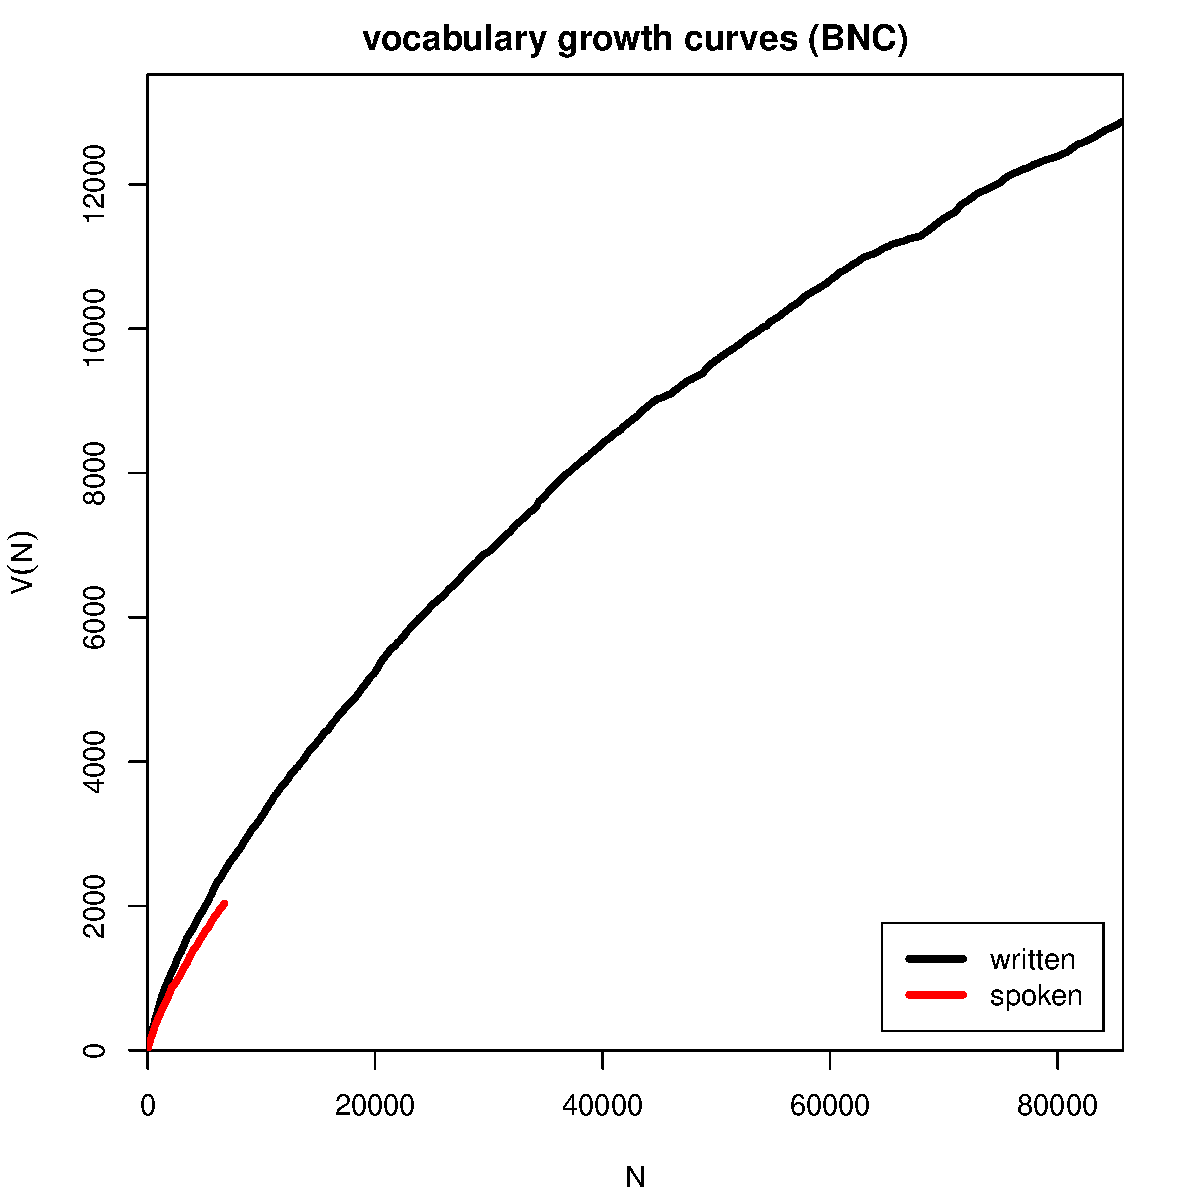
\includegraphics[width=6cm]{img/bare_bncWS_vgc}}
    \end{column}
  \end{columns}
\end{frame}

\begin{frame}[c]
  \frametitle{Are these ``lexical constants'' really constant?}
  %% \framesubtitle{}

  \centering
  \includegraphics[width=11cm]{img/bare_bncS_obs_lexical_constants}
\end{frame}

\begin{frame}[c]
  \frametitle{Simulation: sample size}

  \centering
  \includegraphics[width=11cm]{img/lexconst_sample_size}
\end{frame}

\begin{frame}[c]
  \frametitle{Simulation: frequent lexicalized types}

  \centering
  \includegraphics[width=11cm]{img/lexconst_echo_type}
\end{frame}

%%%%%%%%%%%%%%%%%%%%%%%%%%%%%%%%%%%%%%%%%%%%%%%%%%%%%%%%%%%%%%%%%%%%%%%%
\subsection{LNRE models}

\begin{frame}
  \frametitle{LNRE models}

  \begin{itemize}
  \item State-of-the-art approach to measuring productivity:\\
    \h{LNRE models} \citep{Baayen:01}
    \begin{itemize}
    \item LNRE = Large Number of Rare Events
    \item \citet{Baayen:01} has 887 citations on Google Scholar
    \item[]
    \end{itemize}
  \item Standard implementation: \hh{zipfR} \citep{Evert:Baroni:07}
    \begin{itemize}
    \item 76 citations on Google Scholar
    \item only a few search results for Baayen's \texttt{lexstats} software
    \item[]
    \end{itemize}
  \item LNRE uses various approximations and simplifications to obtain a tractable and elegant model
    \begin{itemize}
    \item LNRE model usually minor component of complex procedure
    \item often applied to very large samples ($N > 1$ M tokens)
    \end{itemize}
  \end{itemize}
\end{frame}

\begin{frame}
  \frametitle{The LNRE population}

  \begin{itemize}
  \item Population: set of $S$ types $w_i$ with occurrence \h{probabilities} $\pi_i$
  \item $S$ = \h{population diversity} can be finite or infinite ($S = \infty$)
  \item Not interested in specific types \so  arrange by decreasing
    probability: $\pi_1\geq \pi_2\geq \pi_3 \geq \cdots$
    \begin{itemize}
    \item[\hand] impossible to determine probabilities of all individual types
    \end{itemize}
  \item Normalization: $\pi_1 + \pi_2 + \ldots + \pi_S = 1$
    \begin{itemize}
    \item[]
    \end{itemize}
  \item \hh{parametric} statistical \hh{model} to describe full population (esp.\ for $S = \infty$),
    i.e.\ a function $i \mapsto \pi_i$
    \begin{itemize}
    \item type probabilities $\pi_i$ cannot be estimated reliably from a sample, but parameters of this function can
    \item NB: population index $i$ $\neq$ Zipf rank $r$
    \end{itemize}
  \end{itemize}
\end{frame}

\begin{frame}
  \frametitle{Zipf-Mandelbrot law as a population model}

  \begin{itemize}
  \item Zipf-Mandelbrot law for type probabilities:
    \[ \pi_i := \frac{C}{(i + b) ^ a} \]
  \item Two free parameters: $a > 1$ and $b \geq 0$
    \begin{itemize}
    \item[\hand] $C$ is not a parameter but a normalization constant,\\
      needed to ensure that $\sum_i \pi_i = 1$
    \end{itemize}
  \item Third parameter: $S > 0$ or $S = \infty$
  \item[]
  \item This is the \h{Zipf-Mandelbrot} population model \citep{Evert:04}
  \end{itemize}
\end{frame}

\begin{frame}
  \frametitle{Samples: type frequency list \& spectrum}

  \ungap[1]
  \begin{center}
    \begin{tabular}[t]{r | rr}
      rank $r$ & $f_r$ & type $i$ \\
      \hline
       1 & 37 &  6 \\
       2 & 36 &  1 \\
       3 & 33 &  3 \\
       4 & 31 &  7 \\
       5 & 31 & 10 \\
       6 & 30 &  5 \\
       7 & 28 & 12 \\
       8 & 27 &  2 \\
       9 & 24 &  4 \\
      10 & 24 & 16 \\
      11 & 23 &  8 \\
      12 & 22 & 14 \\
      \vdots & \vdots & \vdots
    \end{tabular}
    \hspace{2cm}
    \begin{tabular}[t]{r | r}
      $m$ & $V_m$ \\
      \hline
       1 & 83 \\
       2 & 22 \\
       3 & 20 \\
       4 & 12 \\
       5 & 10 \\
       6 &  5 \\
       7 &  5 \\
       8 &  3 \\
       9 &  3 \\
      10 &  3 \\
      \vdots & \vdots \\
      \multicolumn{2}{c}{} \\
      \multicolumn{2}{c}{\hh{sample \#1}}
    \end{tabular}
  \end{center}
\end{frame}

\begin{frame}
  \frametitle{Samples: type frequency list \& spectrum}

  \ungap[1]
  \begin{center}
    \begin{tabular}[t]{r | rr}
      rank $r$ & $f_r$ & type $i$ \\
      \hline
       1 & 39 &  2 \\
       2 & 34 &  3 \\
       3 & 30 &  5 \\
       4 & 29 & 10 \\
       5 & 28 &  8 \\
       6 & 26 &  1 \\
       7 & 25 & 13 \\
       8 & 24 &  7 \\
       9 & 23 &  6 \\
      10 & 23 & 11 \\
      11 & 20 &  4 \\
      12 & 19 & 17 \\
      \vdots & \vdots & \vdots
    \end{tabular}
    \hspace{2cm}
    \begin{tabular}[t]{r | r}
      $m$ & $V_m$ \\
      \hline
       1 & 76 \\
       2 & 27 \\
       3 & 17 \\
       4 & 10 \\
       5 &  6 \\
       6 &  5 \\
       7 &  7 \\
       8 &  3 \\
      10 &  4 \\
      11 &  2 \\
      \vdots & \vdots \\
      \multicolumn{2}{c}{} \\
      \multicolumn{2}{c}{\hh{sample \#2}}
    \end{tabular}
  \end{center}
\end{frame}

\begin{frame}
  \frametitle{Expectation: frequency spectrum}

  \ungap[1]
  \begin{center}
    \only<beamer:0| handout:1>{%
      \begin{tabular}{cc}
        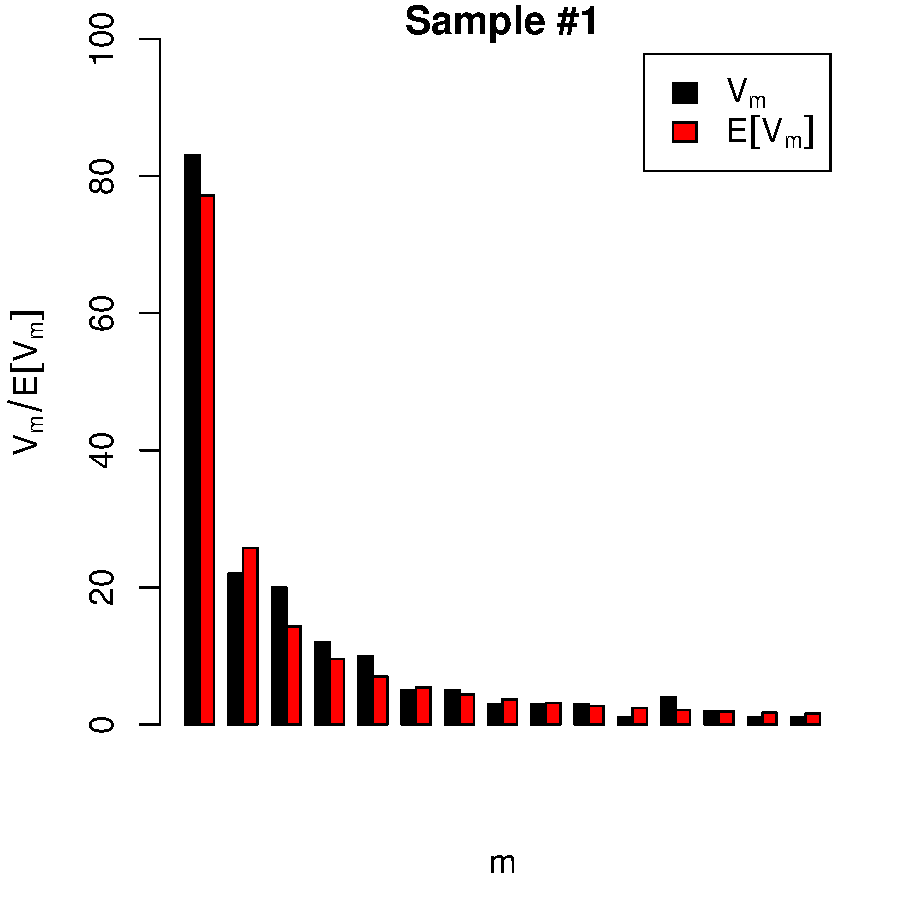
\includegraphics[width=40mm]{img/05-samples-spc-exp-vs-sample-1} &
        \includegraphics[width=40mm]{img/05-samples-spc-exp-vs-sample-2} \\
        \includegraphics[width=40mm]{img/05-samples-spc-exp-vs-sample-3} &
        \includegraphics[width=40mm]{img/05-samples-spc-exp-vs-sample-4} 
      \end{tabular}%
    }%
    \only<beamer:1| handout:0>{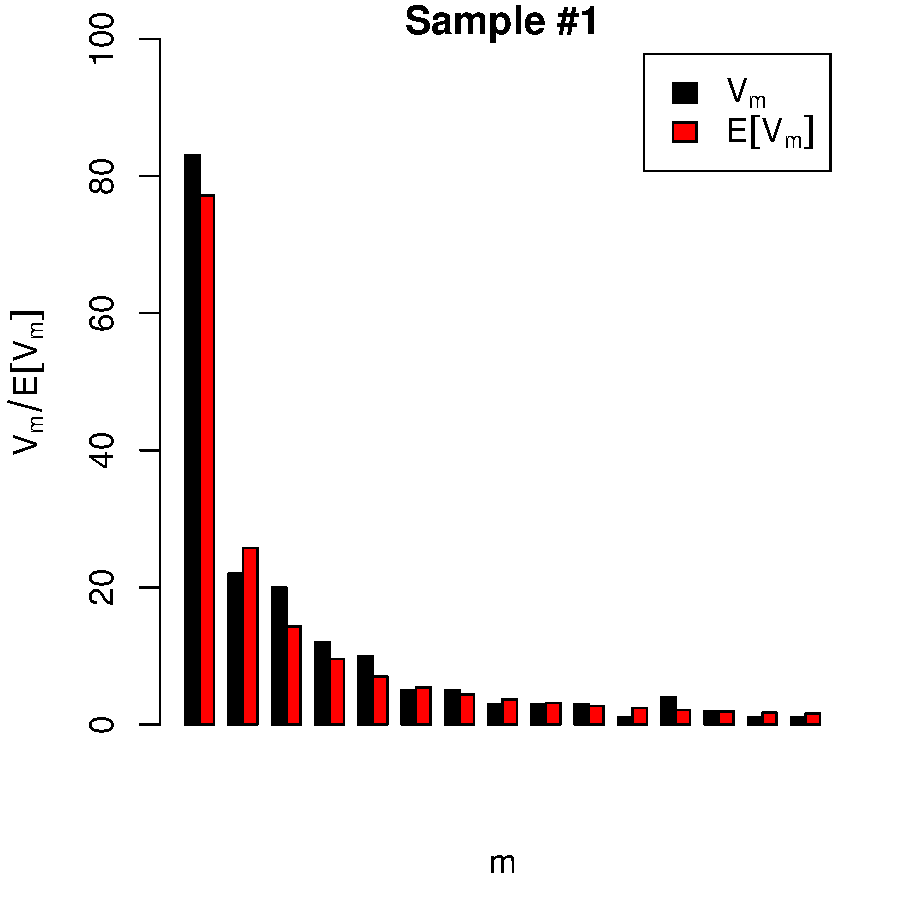
\includegraphics[width=70mm]{img/05-samples-spc-exp-vs-sample-1}}%
    \only<beamer:2| handout:0>{\includegraphics[width=70mm]{img/05-samples-spc-exp-vs-sample-2}}%
    \only<beamer:3| handout:0>{\includegraphics[width=70mm]{img/05-samples-spc-exp-vs-sample-3}}%
    \only<beamer:4| handout:0>{\includegraphics[width=70mm]{img/05-samples-spc-exp-vs-sample-4}}%
  \end{center}
\end{frame}

\begin{frame}
  \frametitle{Expectation: vocabulary growth curve}

  \ungap[1]
  \begin{center}
    \begin{tabular}{c @{} c}
      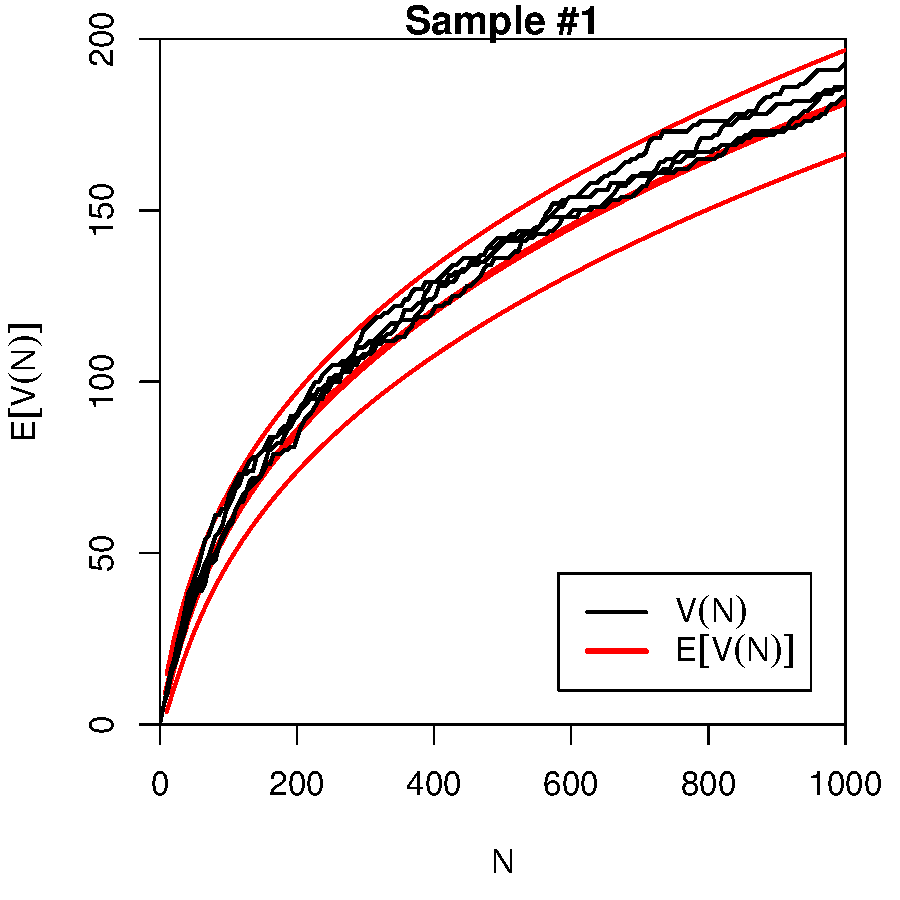
\includegraphics[width=50mm]{img/05-samples-vgc-exp-vs-samples-conf} &
      \includegraphics[width=50mm]{img/05-samples-vgc-V1-exp-vs-samples-conf}
    \end{tabular}
  \end{center}

  ``Confidence intervals'' indicate predicted sampling distribution:%
  \begin{itemize}
  \item[\hand] for 95\% of samples generated by the LNRE model, VGC will fall within the range delimited by the thin red lines
  \end{itemize}
\end{frame}

\begin{frame}[c]
  \frametitle{Extrapolating vocabulary growth}
  
  \centering
  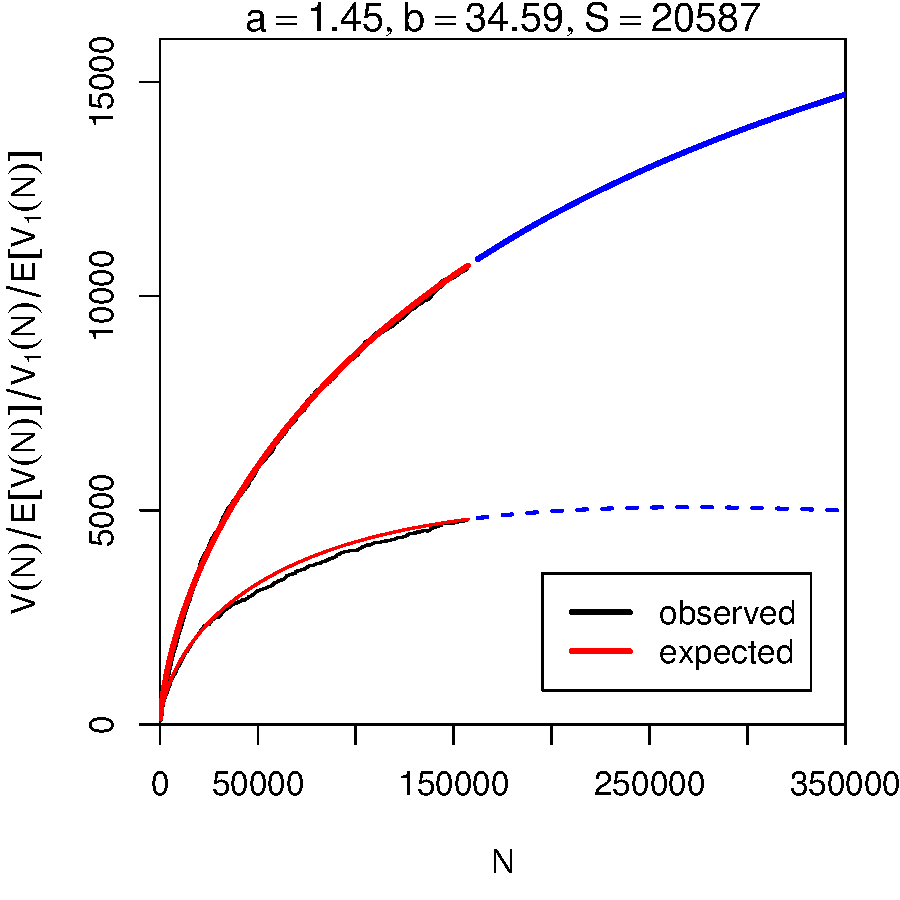
\includegraphics[width=7.5cm]{img/02-samples-ot-vgc-extrapolated}
\end{frame}

\begin{frame}[c]
  \frametitle{Parameter estimation}
  % \framesubtitle{Minimisation of suitable cost function for frequency spectrum}

  \begin{center}
    \begin{tabular}{c @{} c}
      \includegraphics[width=50mm]{img/05-estimation-spc-estimated} &
      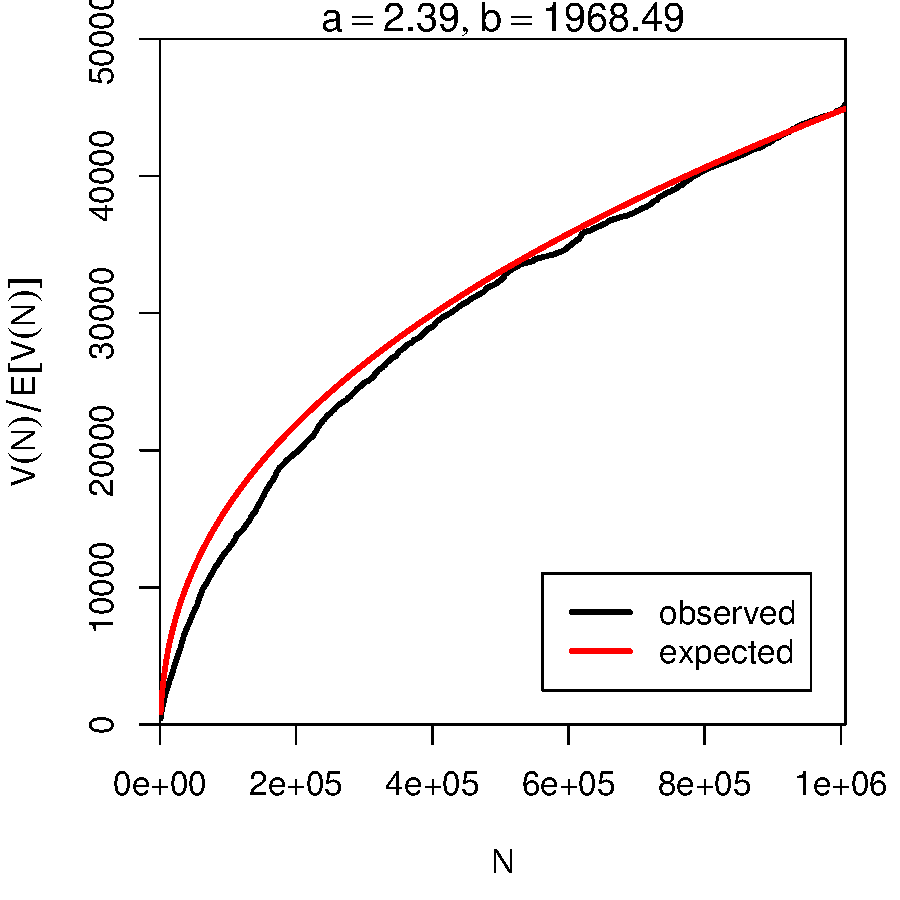
\includegraphics[width=50mm]{img/05-estimation-vgc-estimated} 
    \end{tabular}
  \end{center}

  \ungap[1]
  \begin{itemize}
    \item By trial \& error we found $a=2.0$ and $b=550$
    \item Automatic estimation procedure based on minimisation of suitable cost function: $a=2.39$ and $b=1968$
  \end{itemize}
\end{frame}

\begin{frame}[c]
  \frametitle{Parameter estimation}
  \framesubtitle{ZM model with free parameters $0 < \alpha < 1$ and $B > 0$}
  
  \centering\hspace*{-5mm}%
  \only<beamer:1| handout:1>{\includegraphics[width=12cm]{img/cost_bncBare_chisq_10}}%
  \only<beamer:0| handout:0>{\includegraphics[width=12cm]{img/cost_brownWords_chisq_5}}%
\end{frame}


%%%%%%%%%%%%%%%%%%%%%%%%%%%%%%%%%%%%%%%%%%%%%%%%%%%%%%%%%%%%%%%%%%%%%%%%
\section{Problems}

%%%%%%%%%%%%%%%%%%%%%%%%%%%%%%%%%%%%%%%%%%%%%%%%%%%%%%%%%%%%%%%%%%%%%%%%
\subsection{LNRE models}

\begin{frame}
  \frametitle{Problems of LNRE models}

  \ungap[1]
  \begin{itemize}
  \item Assumption: corpus data = random sample
    \begin{itemize}
    \item[\hand] holds reasonably well for morphological productivity
    \item[\hand] simple but effective \textsc{echo} correction \citep{Baroni:Evert:07a}
    \item[]
    \end{itemize}
  \item<2-> Approximation: independent Poisson sampling
    \begin{itemize}
    \item instead of correct multinomial sampling distribution
    \item[]
    \end{itemize}
  \item<3-> Approximation: multivariate normal distribution of $V$ and $V_m$
    \begin{itemize}
    \item true sampling distribution is completely intractable
    \item[]
    \end{itemize}
  \item<4-> Approximation: continuous type density function $g(\pi)$
    \begin{itemize}
    \item instead of discrete type probabilities of Z-M law
    \item[]
    \end{itemize}
  \item[\So]<5-> Wide-spread irresponsible application of LNRE models to small samples \citep[e.g.][]{Luedeling:Evert:05}
  \end{itemize}
\end{frame}

\begin{frame}
  \frametitle{How reliable are the fitted models?}
  
  Three potential issues:
  \begin{enumerate}
  \item<2-> \h<5->{Model assumptions $\neq$ population}\\
    (e.g.\ distribution does not follow a Zipf-Mandelbrot law)
    \begin{itemize}
    \item[\hand] model cannot be adequate, regardless of parameter settings
    \item[]
    \end{itemize}
  \item<3-> \h<5->{Parameter estimation unsuccessful}\\
    (i.e.\ suboptimal goodness-of-fit to training data)
    \begin{itemize}
    \item[\hand] optimization algorithm trapped in local minimum
    \item[\hand] can result in highly inaccurate model
    \item[]
    \end{itemize}
  \item<4-> Uncertainty due to sampling variation\\
    (i.e.\ training data differ from population distribution)
    \begin{itemize}
    \item[\hand] model fitted to training data, may not reflect true population
    \item[\hand] another training sample would have led to different parameters
    \item[\hand] especially critical for small samples ($N < $ 10,000)
    \end{itemize}
  \end{enumerate}
\end{frame}

\begin{frame}[c]
  \frametitle{Cost functions for German word-formation affixes}

  \centering
  \only<beamer:1| handout:0>{\includegraphics[height=7.5cm]{../plots/cost_bar_linear_m10}}%
  \only<beamer:2| handout:0>{\includegraphics[height=7.5cm]{../plots/cost_bar_mse_m10}}%
  \only<beamer:3| handout:0>{\includegraphics[height=7.5cm]{../plots/cost_bar_chi-square_m10}}%
  \only<beamer:4| handout:0>{\includegraphics[height=7.5cm]{../plots/cost_bar_MLE_m10}}%
  \only<beamer:5| handout:0>{\includegraphics[height=7.5cm]{../plots/cost_bar_MLE_m05}}%
  \only<beamer:6| handout:0>{\includegraphics[height=7.5cm]{../plots/cost_chen_MLE_m05}}%
  \only<beamer:7| handout:0>{\includegraphics[height=7.5cm]{../plots/cost_lein_MLE_m05}}%
  \only<beamer:8| handout:0>{\includegraphics[height=7.5cm]{../plots/cost_sam_MLE_m05}}%
  \only<beamer:0| handout:1>{%
    \hspace*{-5mm}%
    \begin{tabular}{c@{}c}
      \includegraphics[height=6cm]{../plots/cost_bar_mse_m10}
      & \includegraphics[height=6cm]{../plots/cost_bar_MLE_m05}
    \end{tabular}%
  }

\end{frame}

%%%%%%%%%%%%%%%%%%%%%%%%%%%%%%%%%%%%%%%%%%%%%%%%%%%%%%%%%%%%%%%%%%%%%%%%
\subsection{Confidence intervals}

\begin{frame}
  \frametitle{Goodness-of-fit}
  \framesubtitle{\citep[Sec.~3.3]{Baayen:01}}

  \begin{itemize}
  \item Statistics: confidence intervals for population coefficients by inverting hypothesis tests (all $H_0: \mu = x$ with $p > .05$)
  \item<2-> Multivariate normal approximation for $\mathbf{V} = (V, V_1, \ldots, V_k)$:
    \[
      \bigp{\mathbf{V} = \mathbf{v}} \sim
      \frac{
        e^{-\frac12 (\mathbf{v} - \pmb{\mu})^T \pmb{\Sigma}^{-1} (\mathbf{v} - \pmb{\mu})}
      }{\small
        \sqrt{(2\pi)^{k+1} \det \pmb{\Sigma}}
      }
    \]
    with $\pmb{\mu} = (\Exp{V}, \Exp{V_1}, \Exp{V_2}, \ldots)$ and $\pmb{\Sigma}$ = covariance matrix
  \item[]
  \item<3-> Test statistic
    \[
      X^2 = (\mathbf{V} - \pmb{\mu})^T \pmb{\Sigma}^{-1} (\mathbf{V} - \pmb{\mu}) \sim \chi^2_{k + 1}
    \]
  \item<3->[\So] Multivariate chi-squared test of \h{goodness-of-fit}
    \begin{itemize}
    \item[\hand] significant rejection of the LNRE model for $p < .05$
    \end{itemize}
  \end{itemize}
\end{frame}

\begin{frame}[c]
  \frametitle{Confidence sets based on goodness-of-fit test?}

  \centering
  \only<beamer:1| handout:0>{\includegraphics[height=7.5cm]{../plots/cost_lein_MLE_m05}}%
  \only<beamer:2| handout:0>{\includegraphics[height=7.5cm]{../plots/gof_lein_m05}}%
  \only<beamer:3| handout:0>{\includegraphics[height=7.5cm]{../plots/cost_bar_MLE_m05}}%
  \only<beamer:4| handout:0>{\includegraphics[height=7.5cm]{../plots/gof_bar_m05}}%
  \only<beamer:5| handout:0>{\includegraphics[height=7.5cm]{../plots/cost_sam_MLE_m05}}%
  \only<beamer:6| handout:0>{\includegraphics[height=7.5cm]{../plots/gof_sam_m05}}%
  \only<beamer:0| handout:1>{%
    \hspace*{-5mm}%
    \begin{tabular}{c@{}c}
      \includegraphics[height=6cm]{../plots/cost_lein_MLE_m05}
      & \includegraphics[height=6cm]{../plots/gof_lein_m05}
    \end{tabular}%
  }%
  \only<beamer:0| handout:2>{%
    \hspace*{-5mm}%
    \begin{tabular}{c@{}c}
      \includegraphics[height=6cm]{../plots/cost_sam_MLE_m05}
      & \includegraphics[height=6cm]{../plots/gof_sam_m05}
    \end{tabular}%
  }%
\end{frame}

\begin{frame}[c]
  \frametitle{Confidence sets for idealized samples from ZM population}
  \framesubtitle{\primary{\so $X^2$ tests model parameters rather than goodness-of-fit}}

  \centering\ungap[.5]
  \only<beamer:1| handout:0>{\includegraphics[height=7.5cm]{../plots/gof_zm_spc_1000000}}%
  \only<beamer:2| handout:0>{\includegraphics[height=7.5cm]{../plots/gof_zm_spc_50000}}%
  \only<beamer:3| handout:0>{\includegraphics[height=7.5cm]{../plots/gof_zm_spc_10000}}%
  \only<beamer:4| handout:0>{\includegraphics[height=7.5cm]{../plots/gof_zm_spc_5000}}%
  \only<beamer:5| handout:0>{\includegraphics[height=7.5cm]{../plots/gof_zm_spc_2000}}%
  \only<beamer:6| handout:0>{\includegraphics[height=7.5cm]{../plots/gof_zm_spc_1000}}%
  \only<beamer:7| handout:0>{\includegraphics[height=7.5cm]{../plots/gof_zm_spc_500}}%
  \only<beamer:8| handout:0>{\includegraphics[height=7.5cm]{../plots/gof_zm_spc_200}}%
  \only<beamer:0| handout:1>{%
    \hspace*{-5mm}%
    \begin{tabular}{c@{}c}
      \includegraphics[height=6cm]{../plots/gof_zm_spc_5000}
      & \includegraphics[height=6cm]{../plots/gof_zm_spc_200}
    \end{tabular}%
  }%
\end{frame}

%%%%%%%%%%%%%%%%%%%%%%%%%%%%%%%%%%%%%%%%%%%%%%%%%%%%%%%%%%%%%%%%%%%%%%%%%%%%%
\subsection{Bootstrapping}

\begin{frame}
  \frametitle{How reliable are the fitted models?}
  
  Three potential issues:
  \begin{enumerate}
  \item Model assumptions $\neq$ population\\
    (e.g.\ distribution does not follow a Zipf-Mandelbrot law)
    \begin{itemize}
    \item[\hand] model cannot be adequate, regardless of parameter settings
    \item[]
    \end{itemize}
  \item Parameter estimation unsuccessful\\
    (i.e.\ suboptimal goodness-of-fit to training data)
    \begin{itemize}
    \item[\hand] optimization algorithm trapped in local minimum
    \item[\hand] can result in highly inaccurate model
    \item[]
    \end{itemize}
  \item \h{Uncertainty due to sampling variation}\\
    (i.e.\ training data differ from population distribution)
    \begin{itemize}
    \item[\hand] model fitted to training data, may not reflect true population
    \item[\hand] another training sample would have led to different parameters
    \item[\hand] especially critical for small samples ($N < $ 10,000)
    \end{itemize}
  \end{enumerate}
\end{frame}

\begin{frame}
  \frametitle{Bootstrapping}

  \begin{itemize}
  \item<1-> An empirical approach to sampling variation:
    \begin{itemize}
    \item take many random samples from the same population
    \item estimate LNRE model from each sample
    \item analyse distribution of model parameters, goodness-of-fit, etc.
      (mean, median, s.d., boxplot, histogram, \ldots)
    \item problem: how to obtain the additional samples?
    \end{itemize}
  \item<2-> Bootstrapping \citep{Efron:79}
    \begin{itemize}
    \item resample from observed data \emph{with replacement}
    \item this approach is not suitable for type-token distributions
      (resamples underestimate vocabulary size $V$!)
    \end{itemize}
  \item<3-> Parametric bootstrapping
    \begin{itemize}
    \item use fitted model to generate samples, i.e.\ sample from the population described by the model
    \item advantage: ``correct'' parameter values are known
    \end{itemize}
  \end{itemize}
\end{frame}

\begin{frame}
  \frametitle{Bootstrapping}
  \framesubtitle{parametric bootstrapping with 100 replicates, fZM samples for $N = 3467$}

  \ungap[.5]
  \only<beamer:1| handout:1>{\h{Zipfian slope $a = 1 / \alpha$}}%
  \only<beamer:2| handout:0>{\h{Offset $b = (1 - \alpha) / (B\cdot \alpha)$}}%
  \only<beamer:3| handout:0>{\h{fZM probability cutoff $A = \pi_S$}}%
  \only<beamer:4| handout:2>{\h{Goodness-of-fit statistic $X^2$} \secondary{(model not plausible for $X^2 > 11$)}}%
  \only<beamer:5-6| handout:3>{\h{Population diversity $S$}}%
  \ungap[.5]
  \begin{center}
    \only<beamer:1| handout:1>{\includegraphics[width=10cm]{img/05-bootstrap-ultra-alpha}}%
    \only<beamer:2| handout:0>{\includegraphics[width=10cm]{img/05-bootstrap-ultra-B}}%
    \only<beamer:3| handout:0>{\includegraphics[width=10cm]{img/05-bootstrap-ultra-A}}%
    \only<beamer:4| handout:2>{\includegraphics[width=10cm]{img/05-bootstrap-ultra-X2}}%
    \only<beamer:5| handout:0>{\includegraphics[width=10cm]{img/05-bootstrap-ultra-S}}%
    \only<beamer:6| handout:3>{\includegraphics[width=10cm]{img/05-bootstrap-ultra-S-zoomed}}%
  \end{center}
\end{frame}

\begin{frame}[c]
  \frametitle{Sample size matters!}
  \framesubtitle{Brown corpus is too small for reliable LNRE parameter estimation (bare singulars)}

  \centering
  \includegraphics[width=11cm]{img/bare_brown_boot_fzm_a_S}
\end{frame}


%%%%%%%%%%%%%%%%%%%%%%%%%%%%%%%%%%%%%%%%%%%%%%%%%%%%%%%%%%%%%%%%%%%%%%

\begin{frame}[c]
  \begin{center}
    \counterpoint{\huge Thank you!}
  \end{center}
\end{frame}


%%%%%%%%%%%%%%%%%%%%%%%%%%%%%%%%%%%%%%%%%%%%%%%%%%%%%%%%%%%%%%%%%%%%%%
%% References (if any)

\frame[allowframebreaks]{
  \frametitle{References}
  \bibliographystyle{natbib-stefan}
  \begin{scriptsize}
    \bibliography{stefan-publications,stefan-literature}
  \end{scriptsize}
}

\end{document}
